\section{Návrh zapojení a tvorba DPS}
\label{sec:ridici-jednotka-schema-a-dps}
    Řídicí jednotka je tvořena jednou speciálně navrženou DPS, která kromě samotného mikrokontroléru obsahuje také měnič napětí typu buck ke snížení napájecího napětí externího zdroje na hodnotu \qty{5.2}{V}. Toto napětí je pak dále používáno pro napájení samotného mikrokontroléru řídicí jednotky a zároveň je vyvedeno na konektor pro připojení periferií. Blokové schéma na úrovni logických bloků v~rámci jedné DPS je na obr.~\ref{fig:ridici-jednotka-blokove-schema}, jednotlivým částem se blíže věnují další kapitoly. Celé schéma je k~dispozici v~příloze~\ref{priloha:schema-ridici-jednotka}.

    \begin{figure}[h!]
        \centering
        % trim=left bottom right top
        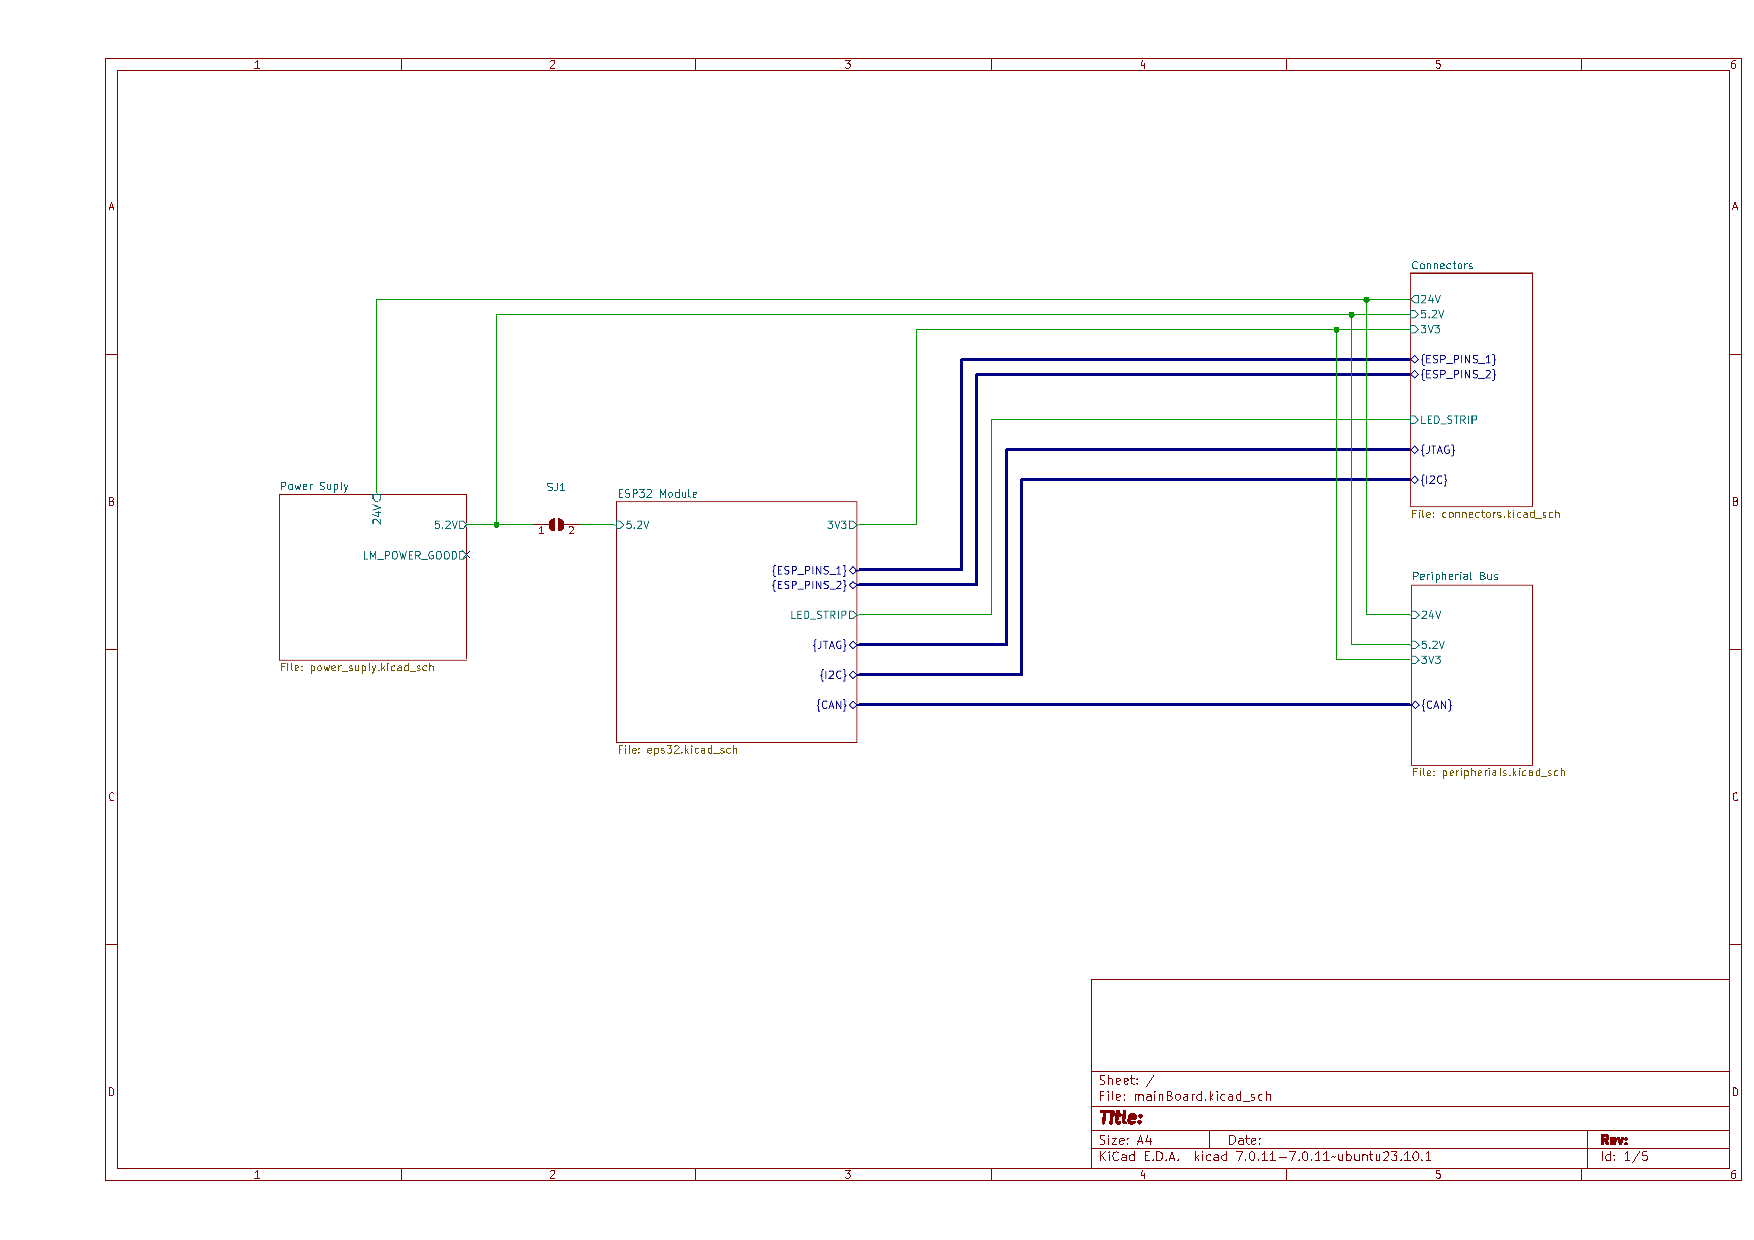
\includegraphics
        [
            width=\textwidth, 
            page=1, 
            trim=4.5cm 9cm 3cm 4cm, 
            clip
        ]{obrazky/exportovane/main-board-schematic.pdf}
        \caption{Blokové schéma řídicí jednotky. Vytvořeno v~KiCad 7.0.}
        \label{fig:ridici-jednotka-blokove-schema}
    \end{figure}
    % TODO: jiná blokovka než z kicadu

    \subsection{Zapojení ESP32 modulu}
    \label{sec:ridici-jendotka-esp32-modul}
    % TODO: Označení součástek ve schématu se změnilo
        Při tvorbě schématu bylo vycházeno z~dokumentace výrobce~\cite{esp32-wroom-32e-datasheet} a také ze schématů různých existujících vývojových desek. K~zajištění správné a spolehlivé funkce modulu je potřeba dodržet několik věcí. Výřez schématu obsahující potřebné doplňující obvody pro ESP32 modul je na obr.~\ref{fig:ridici-jednotka-esp-obvody}.

        \begin{figure}[h!]
            \centering
            % trim=left bottom right top
            \includegraphics
            [
                width=0.9\textwidth, 
                page=2, 
                trim=2.5cm 8.5cm 15.5cm 2cm, 
                clip
            ]{obrazky/exportovane/main-board-schematic.pdf}
            \caption{Podpůrné obvody pro modul ESP32-WROOM-E. Vytvořeno v~KiCad 7.0.}
            \label{fig:ridici-jednotka-esp-obvody}
        \end{figure}

        Na napájecí pin (3V3) je třeba přivést stabilní napětí a opatřit ho blokovacími kondenzátory (C1, C3). Ke snížení napětí z~původních \qty{5,2}{V} na požadovaných \qty{3,3}{V} je použit lineární regulátor TLV76133 (U4). %TODO jiný part number asi
        
        % TODO: Čas ke stabilizaci bude mnohem větší než 50 us. Nejprve totiž musí naběhnout 3V3, což trvá dle datasheetu TLV76133 trvá cca 500 us. Taky bys správně měl zohlednit i náběh 5V2, což je 3 ms.
        Dále je potřeba přivést kladné napětí na povolovací pin (EN). Z~dokumentace vyplývá, že by mělo být přivedeno až po ustálení napájecí linky. Uvedený čas nutný ke stabilizaci je roven \(t_{STBL}=\qty{50}{\micro\second}\)~\cite{esp32-datasheet}. Požadované zpoždění zajistí RC článek (R1, C2) s~časovou konstantou \(\tau\):
        \begin{equation}
            \tau=R_{1}C_{2}=\qty{10}{\kilo\ohm}\cdot \qty{1}{\micro\farad}=\qty{10}{\milli\second}
        \end{equation} 
        Jak je vidět, byla zvolena dostatečná návrhová rezerva. 

        Pro možnost resetu zařízení a vstupu do bootloaderu byla doplněna také dvě tlačítka (SW1, SW2).



    \subsection{Napájecí obvod}
        \label{sec:ridici-jendotka-napajeci-obvod}
        % \textit{TODO: schéma, výpočet hodnot součástek}
        Pro napájení celého zařízení je použit externí zdroj stejnosměrného napětí \qty{24}{V} a toto napětí je tak0 rozvedeno všem připojeným periferiím. Pro většinu komponent je ale nutné napětí snížit. K~tomuto účelu byl navržen DC/DC měnič typu buck s~požadovaným výstupním napětím \qty{5.2}{V}. Existuje celá řada čipů vyvinutých pro tento účel. Aplikace v~tomto zařízení je specifická svými požadavky na výstupní proud, zatímco samotná řídicí jednotka nebude odebírat velký proud, není jasně dané, kolik periferí a s~jakými výkonovými požadavky uživatel k~systému připojí. Navržený měnič tak musí fungovat v~širším rozsahu proudů (řádově od desítek mA po jednotky A) a to s~co nejlepší účinností. 
        
        \begin{figure}[h!]
            \centering
            % trim=left bottom right top
            \includegraphics
            [
                width=\textwidth, 
                page=2, 
                trim=2.2cm 8.5cm 13cm 1.3cm, 
                clip
            ]{obrazky/exportovane/ukazky-do-textu.pdf}
            \caption{Napájecí obvod řídicí jednotky. Vytvořeno v~KiCad 7.0.}
            \label{fig:ridici-jednotka-napajeni-simp}
        \end{figure}

        
        Aby bylo vyhověno zmíněným požadavkům a zachována návrhová rezerva, byl jako základ buck měniče zvolen čip LM5148~\cite{lm5148-datasheet}. Jedná se o~moderní součástku firmy Texas Instruments s~velkou výkonovou rezervou. Tento čip funguje pouze jako buck kontrolér a zapojení je potřeba doplnit zapojení dvěma externími MOSFET tranzistory, většina tepelných ztrát vzniká právě na nich, čímž se sníží ohřev samotného čipu a generované teplo se lépe rozloží. Na volbě tranzistorů závisí také výsledná účinnost měniče. Při návrhu zapojení této součástky byl použit nástroj Webench Power Designer~\cite{webench-power-designer}, který podle zadaných porametrů navrhne konkrétní schéma zapojení, provede simulaci a zobrazí grafy upravené na míru zadaným hodnotám. Tento nástroj uvádí přibližnou účinnost zapojení jako \qty{88}{\percent}. V~navrženém schématu bylo posléze provedeno několik změn, aby vše odpovídalo požadavkům uvedeným v~katalogovém listu součástky~\cite{lm5148-datasheet}. Kompletní schéma zapojení spolu s odkazy k relevantním kapitolám katalogového listu se nachází v příloze~\ref{priloha:schema-ridici-jednotka-napajeci-obvod}, pro přibližnou představu pak postačí zjednodušené schéma na obr.~\ref{fig:ridici-jednotka-napajeni-simp}. 

        \textit{TODO: výpočty by asi bylo dobré uvést co?}

    \subsection{Deska plošných spojů}
        Ačkoliv se jedná o relativně jednoduchou DPS, je potřeba při návrhu dbát jistých pravidel a doporučení. Modul ESP32 je vybaven anténou a volba jeho umístění na DPS je rozhodujícím faktorem pro sp8vnou funkci antény. Další částí vyžadující správný návrh rozložení a propojení součástek je pak buck měnič. 
        
        \begin{figure}[!ht]
            \centering
            \begin{tikzpicture}
                % Include the image
                \node[anchor=south west,inner sep=0] (image) at (0,0) {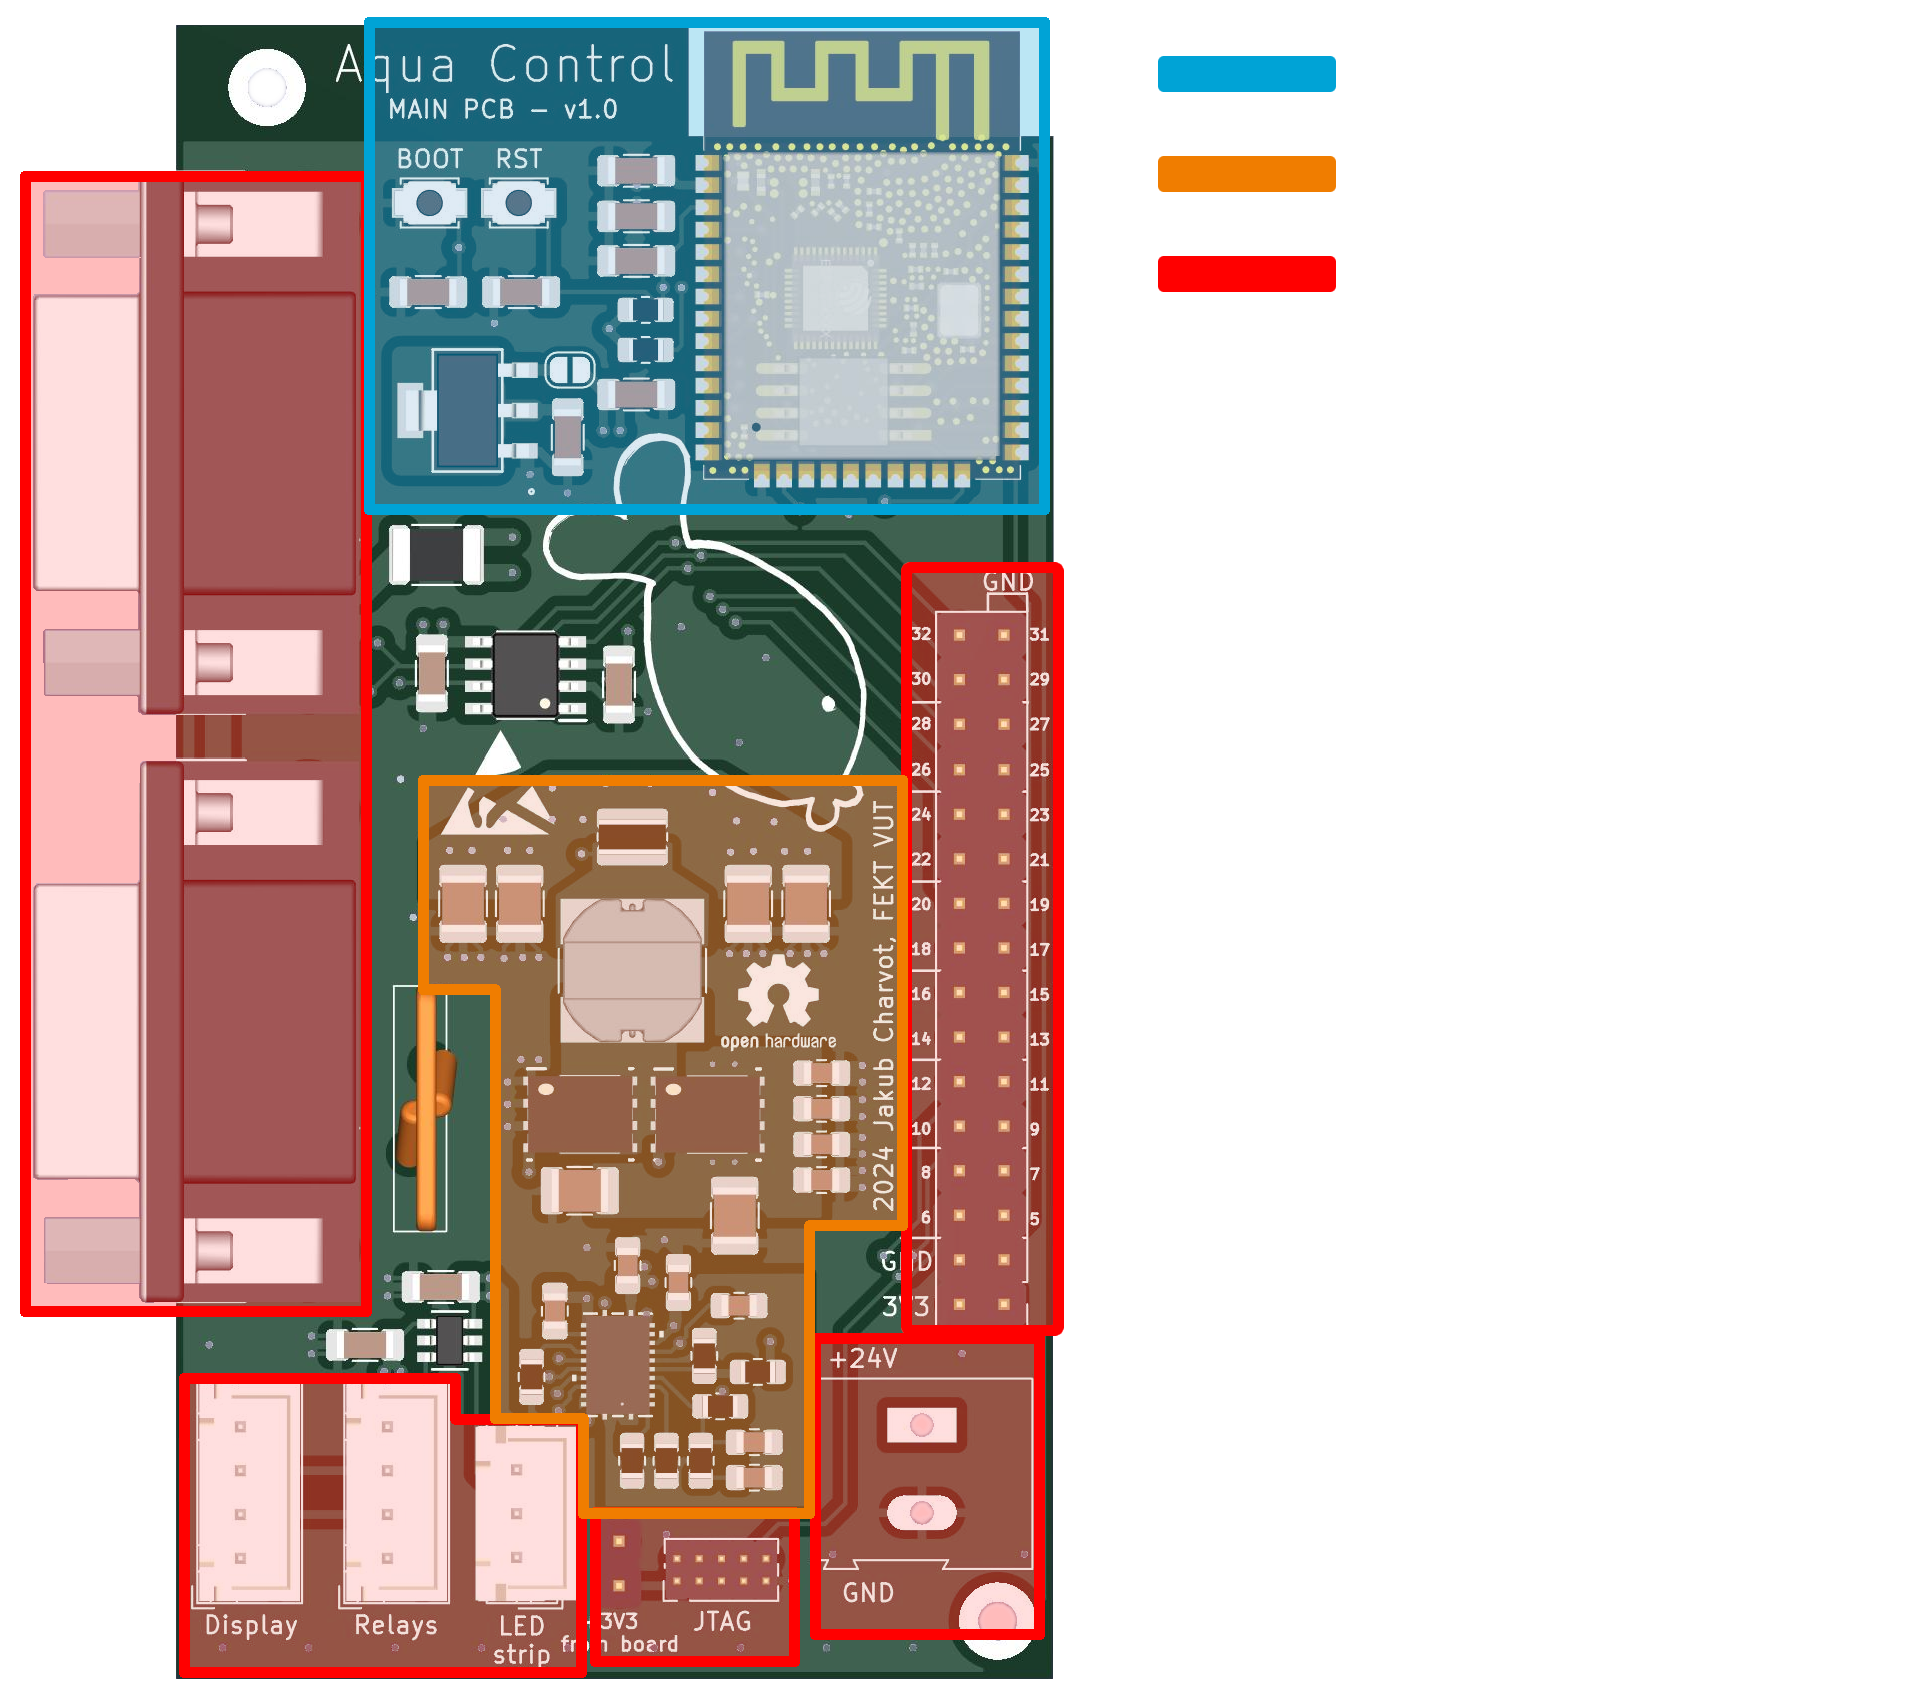
\includegraphics[width=0.8\textwidth]{obrazky/dps/mainBoard-3d-top-popis.png}};
                
                % \draw[->,thick] (0,0) -- (1,9.4);
                \node[anchor=south west,inner sep=0,color=red] at (0.5,9.7)  {1.};
                \node[anchor=south west,inner sep=0,color=red] at (0.6,1.3)  {2.};
                \node[anchor=south west,inner sep=0,color=red] at (4.2,-0.4)  {3.};
                \node[anchor=south west,inner sep=0,color=red] at (6.8,1.3)  {4.};
                \node[anchor=south west,inner sep=0,color=red] at (6.8,5)  {5.};
                % legend
                \node[anchor=south west,inner sep=0] (leg-blu) at (8.5,10)  {MCU};
                \node[anchor=south west,inner sep=0] (leg-ora) at (8.5,9.32) {buck měnič napětí};
                \node[anchor=south west,inner sep=0] (leg-red) at (8.5,8.64) {Konektory:};

                \node[below left=0.8 and 0.6 of leg-red, anchor=south west] (kon1) {1. Ovládané periferie};
                \node[below left=0.6 and 0.0 of kon1, anchor=south west] (kon2) {2. Externí moduly};
                \node[below left=0.6 and 0.0 of kon2, anchor=south west] (kon3) {3. Programování};
                \node[below left=0.6 and 0.0 of kon3, anchor=south west] (kon4) {4. Vstup napájení};
                \node[below left=0.6 and 0.0 of kon4, anchor=south west] (kon5) {5. Testování, rozšíření};
                % \node[anchor=south west,inner sep=0,color=red] {2.};
                % \node[anchor=south west,inner sep=0,color=red] {3.};
                % \node[anchor=south west,inner sep=0,color=red] {4.};
                % \node[anchor=south west,inner sep=0,color=red]          {5.};
            \end{tikzpicture}
            \caption{Vizualizace DPS řídicí jednotky s vyznačením jednotlivých částí.}
            \label{fig:ridici-jendotka-dps-popis}
        \end{figure}

        Prvním krokem návrhu je volba počtu vrstev a jejich funkce. Vyšší počet vrstev nabízí více prostoru pro vedení cest a také umožňuje vedení napájecích napětí pomocí rozlitých měděných polygonů, čímž se zároveň zlepší vlastnosti zařízení z hlediska EMC. Zvolený výrobce (JLC PCB~\cite{jlcpcb}) nabízí výrobu desek s jednou až dvaceti vrstvami mědi. Byla zvolena čtyřvrstvá deska, která je pro danou aplikaci dostatečná a stále se nachází v přijatelné cenové skupině výrobce. Rozložení a funkce vrstev jsou vyobrazeny na obr.~\ref{fig:ridici-jednotka-stackup-dps}.

        Pro optimální fukci Wi-Fi antény výrobce doporučuje umístit ESP32 modul do pravého horního rohu DPS tak, aby se pod anténou nenacházela vrsta mědi a nejlépe ani samotná deska~\cite{esp32-hw-guidelines}. Na obr.~\ref{fig:ridici-jendotka-dps-popis} je zobrazen výsledný návrh DPS, v modře vyznačené oblasti lze vidět, že tyto požadavky byly splněny. Vedle ESP32 modulu se nachází související součástky popsané v kapitole~\ref{sec:ridici-jendotka-esp32-modul}.

        \begin{figure}[h!]
            \centering
            % trim=left bottom right top
            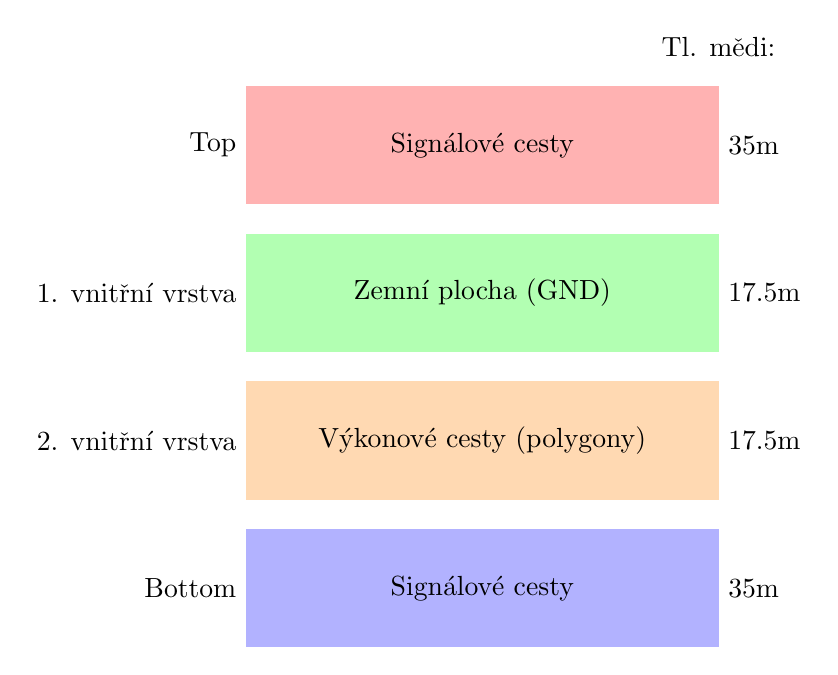
\begin{tikzpicture}[scale=1.5]

                % Layers
                \fill[red!30]    (0,3.75)   rectangle (4,4.75);
                \fill[green!30]  (0,2.5)    rectangle (4,3.5);
                \fill[orange!30] (0,1.25)   rectangle (4,2.25);
                \fill[blue!30]   (0,0)      rectangle (4,1);
                

                % Layer labels
                \node at (2,4.25) {Signálové cesty};
                \node at (2,3) {Zemní plocha (GND)};
                \node at (2,1.75) {Výkonové cesty (polygony)};
                \node at (2,0.5) {Signálové cesty};

                \node[anchor=east] at (0,4.25) {Top};
                \node[anchor=east] at (0,3)    {1. vnitřní vrstva};
                \node[anchor=east] at (0,1.75) {2. vnitřní vrstva};
                \node[anchor=east] at (0,0.5)  {Bottom};

                \node[anchor=north] at (4,5.25) {Tl. mědi:};
                \node[anchor=west] at (4,4.25) {\qty{35}{\micro m}};
                \node[anchor=west] at (4,3)    {\qty{17.5}{\micro m}};
                \node[anchor=west] at (4,1.75) {\qty{17.5}{\micro m}};
                \node[anchor=west] at (4,0.5)  {\qty{35}{\micro m}};
                
                % Comments
                % \draw[<-,thick] (0,3.75)    -- +(0.5,-0.5) node[below] {Bottom Layer};
                % \draw[<-,thick] (0,2.5)     -- +(0.5,-0.5) node[below] {Inner Layer 2};
                % \draw[<-,thick] (0,1.25)    -- +(0.5,-0.5) node[below] {Inner Layer 1};
                % \draw[<-,thick] (0,0)       -- +(0.5,-0.5) node[below] {Top Layer};
                
                \end{tikzpicture}
            \caption{Rozložení vrstev DPS řídicí jednotky.}
            \label{fig:ridici-jednotka-stackup-dps}
        \end{figure}


        \subsubsection{Měnič napětí}
            \textit{TODO: Zde popis návrhu, zdroje, obrázky}
            \textit{Q: Jak moc do detailu?}

   

    \section{Konektivita}
        Řídicí jednotka je vybavena několika konektory, jak je opět možno vidět na obr.~\ref{fig:ridici-jendotka-dps-popis}. Na levé straně DPS (značeno 1.) se nachází konektory pro připojení periferií připravené pro montáž do panelu, kde pak budou přístupné uživateli. Ostatní vyznačené konektory slouží pro připojení externích modulů v rámci hlavního šasi (viz blokové schéma na obr.~\ref{fig:blokove-schema}) popř. pro programování a testování, nebudou tedy volně přístupné uživateli.

        Abychom předešli poškození zařízení při nevhodném zacházení uživatelem, je potřeba pro volně dostupné konektory přidat dodatečnou ochranu~\cite{altium-circuit-protection}. Jak je vidět na obr.~\ref{fig:komunikacni-rozhr-dsub-pinout}, konektor pro periferie sdružuje jak datovou komunikaci, tak i napájení. Ochranu diferenční datové linky zajistí samotný CAN řadič, který je určen pro průmyslové použití a obsahuje zabudovanou ochranu jak proti zkratu datové linky s napájením či zemí, tak proti ESD~\cite{ata-datasheet}. 

        \begin{figure}[h!]
            \centering
            % trim=left bottom right top
            \includegraphics
            [
                width=0.9\textwidth, 
                page=5, 
                trim=8.5cm 7.6cm 7.5cm 3cm, 
                clip
            ]{obrazky/exportovane/main-board-schematic.pdf}
            \caption{Zapojení a ochrana konektorů. Vytvořeno v~KiCad 7.0.}
            \label{fig:ridici-jednotka-konektory}
        \end{figure}
        % TODO: nove schema dodat

        Co se týče napájecích vodičů, každý z nich je ošetřen vratnou pojistkou (ang. polyfuse) dimenzovanou podle předpokládaného maximálního odběru zařízení. Při překročení tohoto proudu, např. z důvodu zkratu v některé z periferií, pojistka sepne a proud v obvodu omezí na minimum. Schéma zapojení konektorů spolu s hodnotami vratných pojistek se nachází na obr.~\ref{fig:ridici-jednotka-konektory}.


            